\documentclass{article}
\usepackage{amsmath}
\usepackage{amsthm}
\usepackage{amsfonts}
\usepackage{amssymb}
\usepackage{bbold}
\usepackage{dsfont}
\usepackage{graphicx}
\usepackage{cleveref}
\usepackage{bm}
\usepackage{booktabs}
\usepackage{siunitx}
\usepackage{xcolor}
\usepackage{pdfpages}
\usepackage[utf8]{inputenc}
\usepackage[english]{babel}
\newtheorem{definition}{Definition}
\newtheorem{example}{Example}
\newcommand{\exP}[1]{\mathrm{e}^{#1}}
\newcommand{\dif}{\mathrm{d}}
\renewcommand{\vec}[1]{\mathbf{#1}}
\newcommand{\pdagger}{{\phantom{\dagger}}}
\newcommand{\state}[1]{\vert #1\rangle}
\newcommand{\cstate}[1]{\langle #1\vert}
\newcommand{\tr}[1]{\mathrm{tr}\left\{#1\right\}}
\newcommand{\trs}[2]{\, \mathrm{tr}_{#1}\{#2\}}
\newcommand{\expc}[3]{\langle #1\vert #2 \vert #3\rangle}
\usepackage[doi=false,url=false,isbn=false,backend=bibtex,style=nature,natbib=true,sorting=none]{biblatex}
\bibliography{bib.bib}
\usepackage{geometry}
\geometry{
	a4paper,
	total={170mm,257mm},
	left=15mm,
	right=15mm,
	top=15mm,
}
\begin{document}
\title{Report 26: TTHEOM results, variation of electron-vibrational coupling}
\maketitle
\section{Parameters}
\begin{itemize}
	\item $N=1\times 3$
	\item $\varepsilon_0 = -\SI{240}{\milli\electronvolt}$
	\item $\omega_0 = \SI{100}{\milli\electronvolt}$
	\item $t_0=\SI{40}{\milli\electronvolt}$
	\item $\lambda_0=\SI{4}{\milli\electronvolt}$
	\item $\lambda_1=\SI{0.4}{\milli\electronvolt}$
	\item $\Gamma_0=\SI{10}{\milli\electronvolt}$
	\item $k_B T=\SI{25}{\milli\electronvolt}$
	\item $t_1\in[1,2.5,5,7.5]t_0$
	\item $V\in[0.25,0.5,0.75]\SI{}{\volt}$
\end{itemize}
\section{$t_1=t_0=\SI{40}{\milli\electronvolt}$}
\subsection{Charge currents}
\begin{figure}[!h]
	\centering
	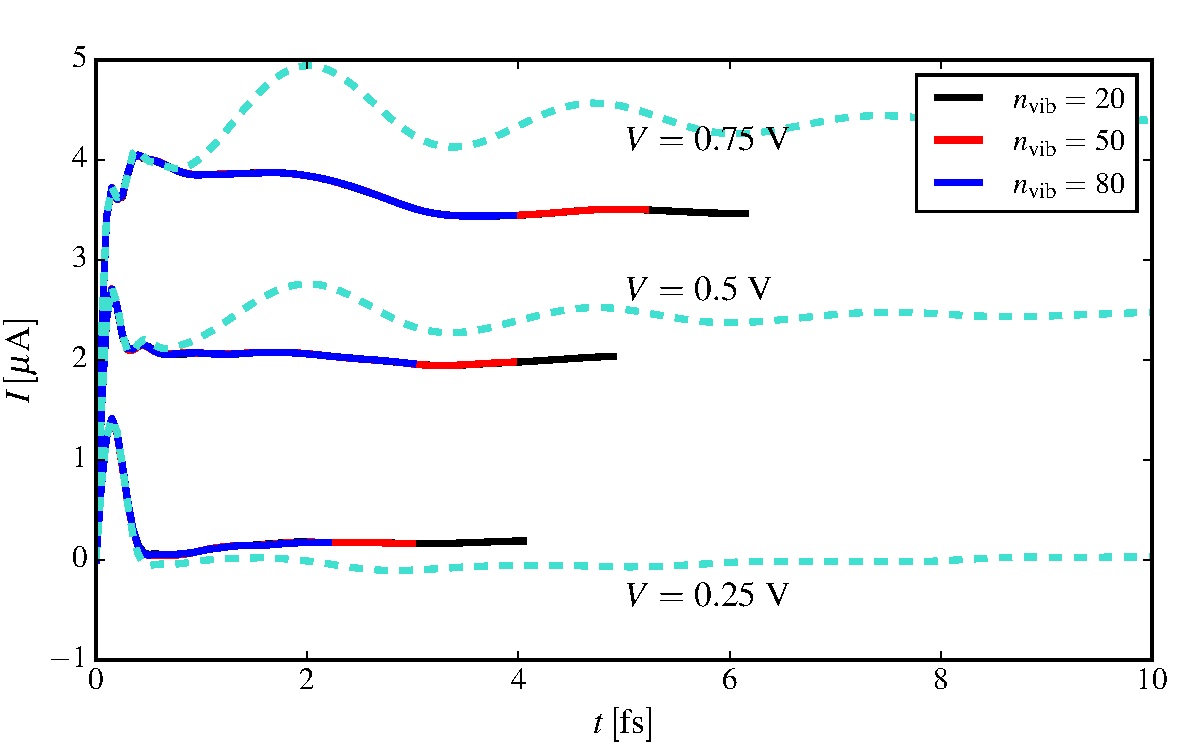
\includegraphics[width=0.8\textwidth]{figs/L1x3_t1_10_tamen_cur_P_Vvar_nVar_tol1e-3.pdf}
	\caption{Charge current for varying voltage. Dashed line denotes result for $t_1=\lambda_1=0$.}
\end{figure}
\clearpage
\subsection{Spin selectivity}
\begin{figure}[!h]
	\centering
	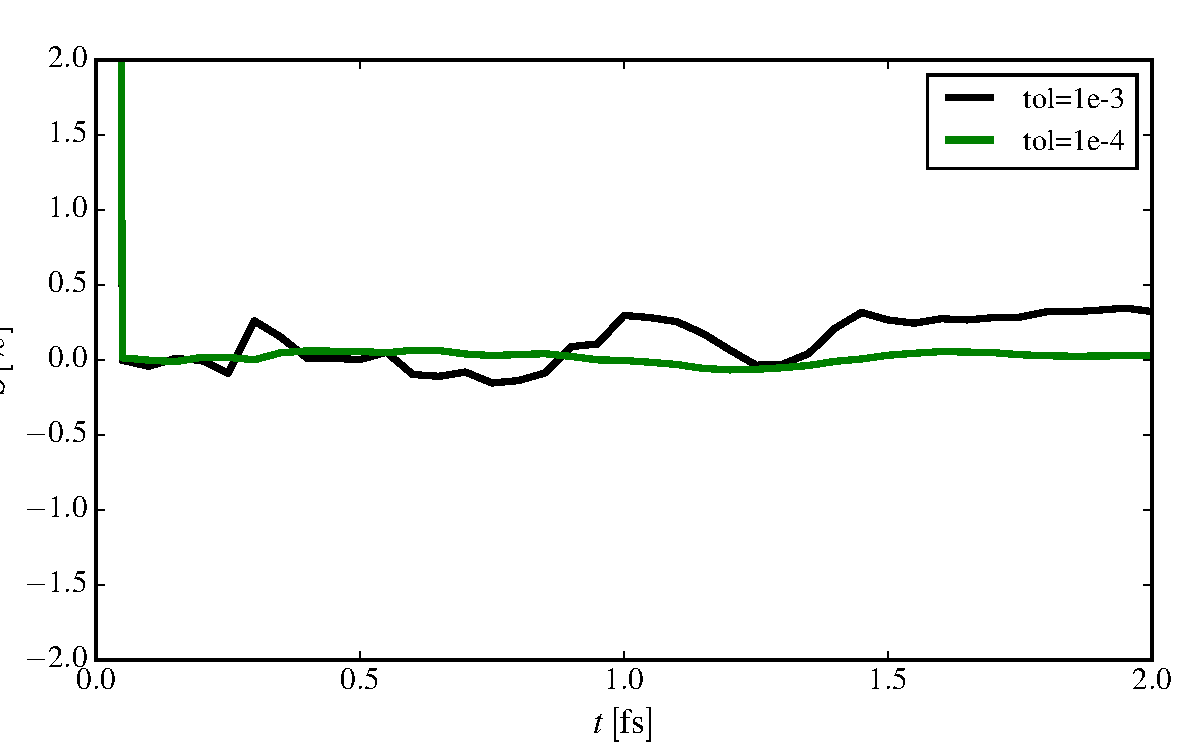
\includegraphics[width=0.5\textwidth]{figs/L1x3_t1_10_tamen_nvib20_SP_V10_tolVar.pdf}
	\caption{$n_\mathrm{vib}=20$.}
\end{figure}
\begin{figure}[!h]
	\centering
	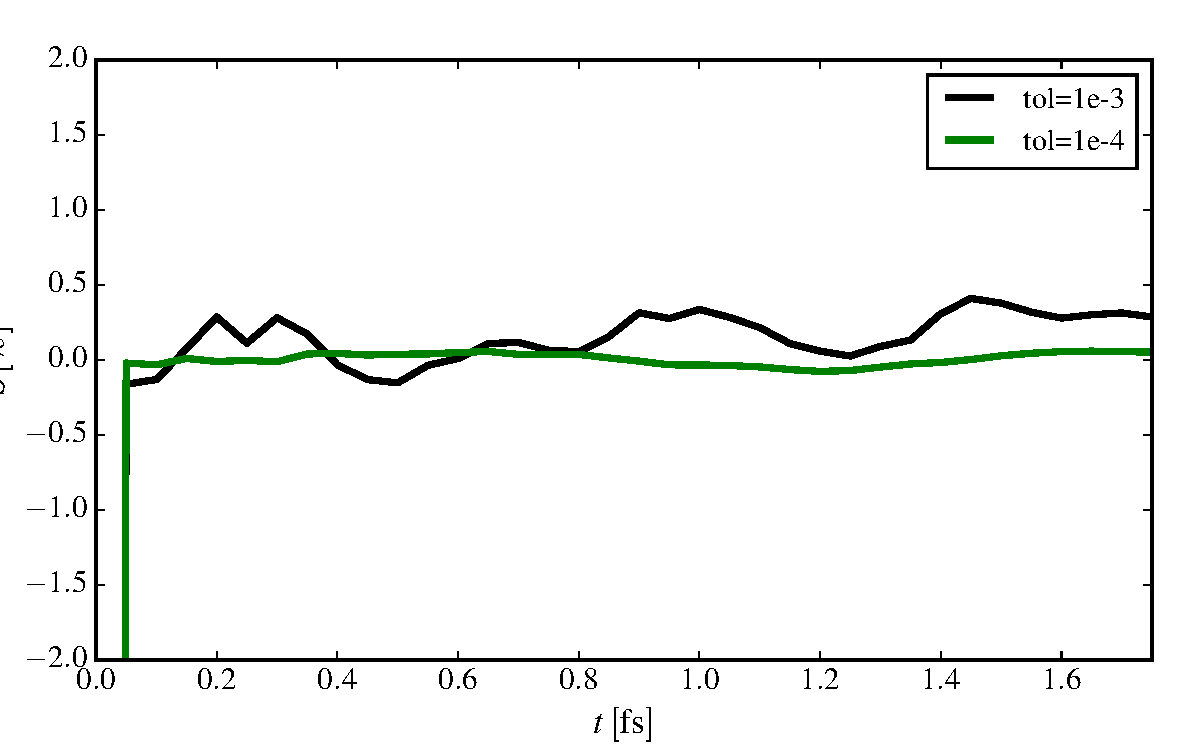
\includegraphics[width=0.5\textwidth]{figs/L1x3_t1_10_tamen_nvib50_SP_V10_tolVar.pdf}
	\caption{$n_\mathrm{vib}=50$.}
\end{figure}
\begin{figure}[!h]
	\centering
	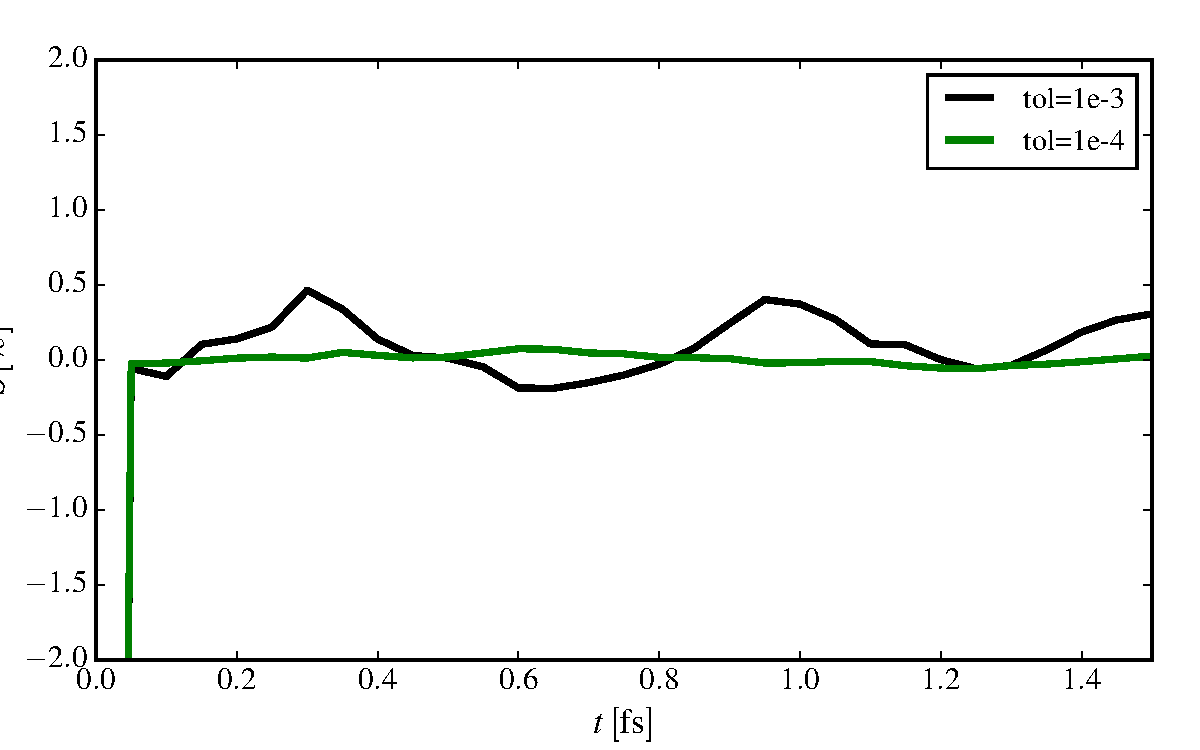
\includegraphics[width=0.5\textwidth]{figs/L1x3_t1_10_tamen_nvib80_SP_V10_tolVar.pdf}
	\caption{$n_\mathrm{vib}=80$.}
\end{figure}
\clearpage
\subsection{Vibrational occupation number}
\begin{figure}[!h]
	\centering
	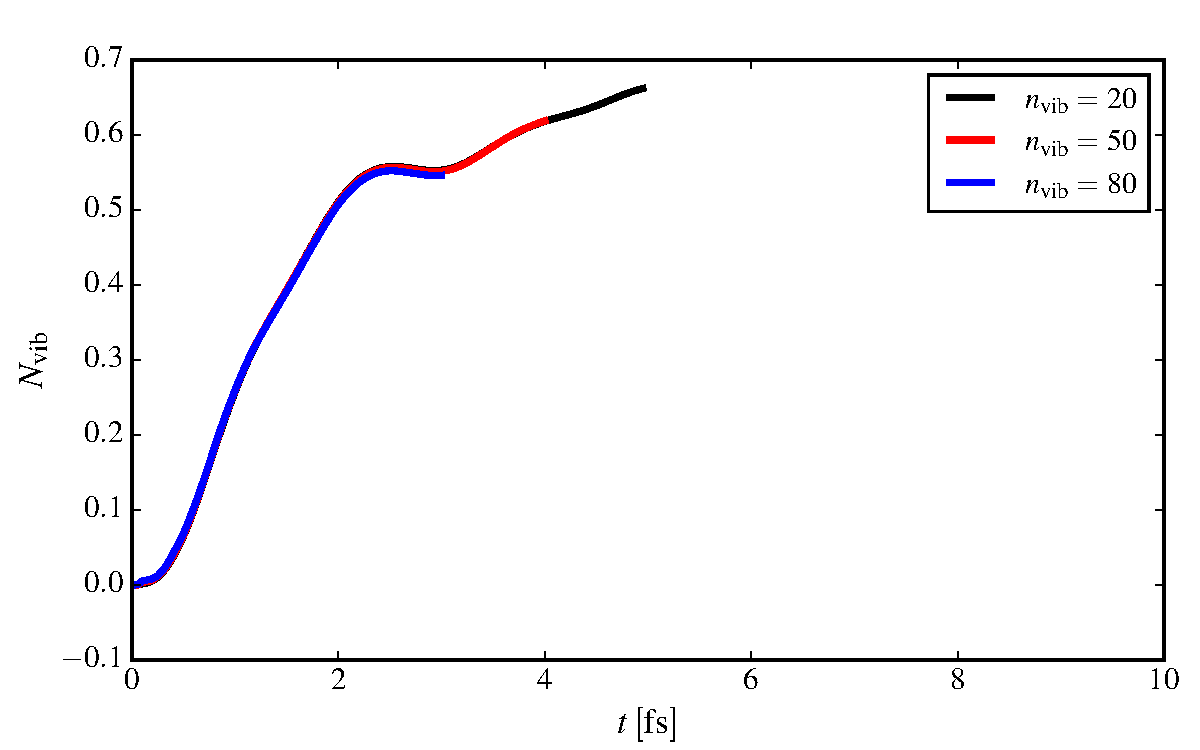
\includegraphics[width=0.75\textwidth]{figs/L1x3_t1_10_tamen_Nvib_P_Vvar_nVar_tol1e-3.pdf}
	\caption{$V=\SI{0.5}{\volt}$, tol$\ =10^{-3}$.}
\end{figure}
\subsection{Maximal rank}
\begin{figure}[!h]
	\centering
	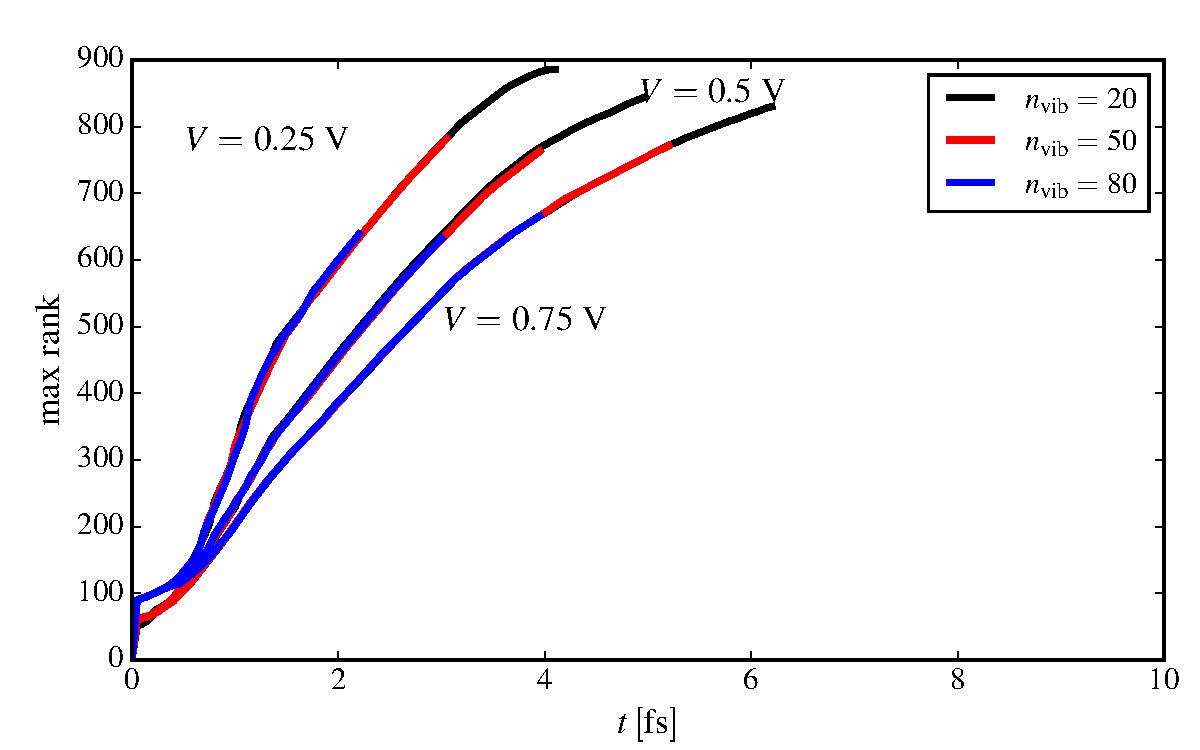
\includegraphics[width=0.75\textwidth]{figs/L1x3_t1_10_tamen_maxRank_P_Vvar_nVar_tol1e-3.pdf}
	\caption{tol$\ =10^{-3}$.}
\end{figure}
\clearpage
\section{$t_1=\SI{100}{\milli\electronvolt}$}
\subsection{Charge currents}
\begin{figure}[!h]
	\centering
	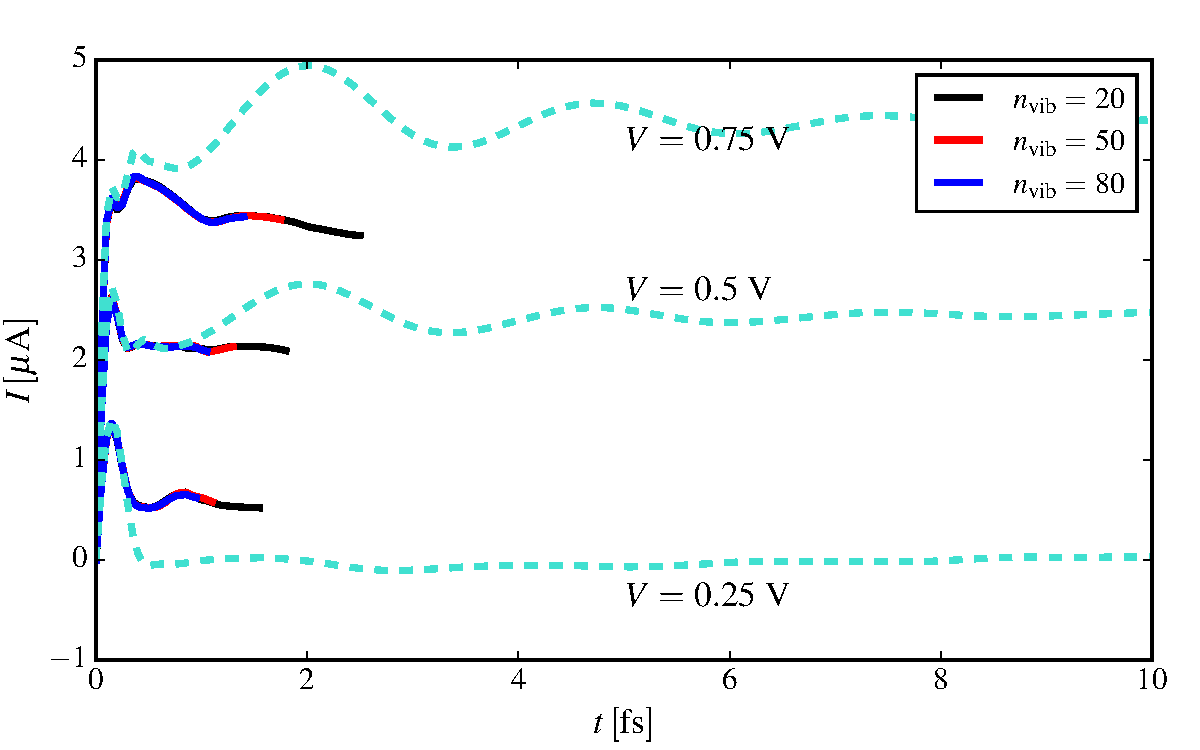
\includegraphics[width=0.8\textwidth]{figs/L1x3_t1_25_tamen_cur_P_Vvar_nVar_tol1e-3.pdf}
	\caption{Charge current for varying voltage. Dashed line denotes result for $t_1=\lambda_1=0$.}
\end{figure}
\subsection{Spin selectivity}
\begin{figure}[!h]
	\centering
	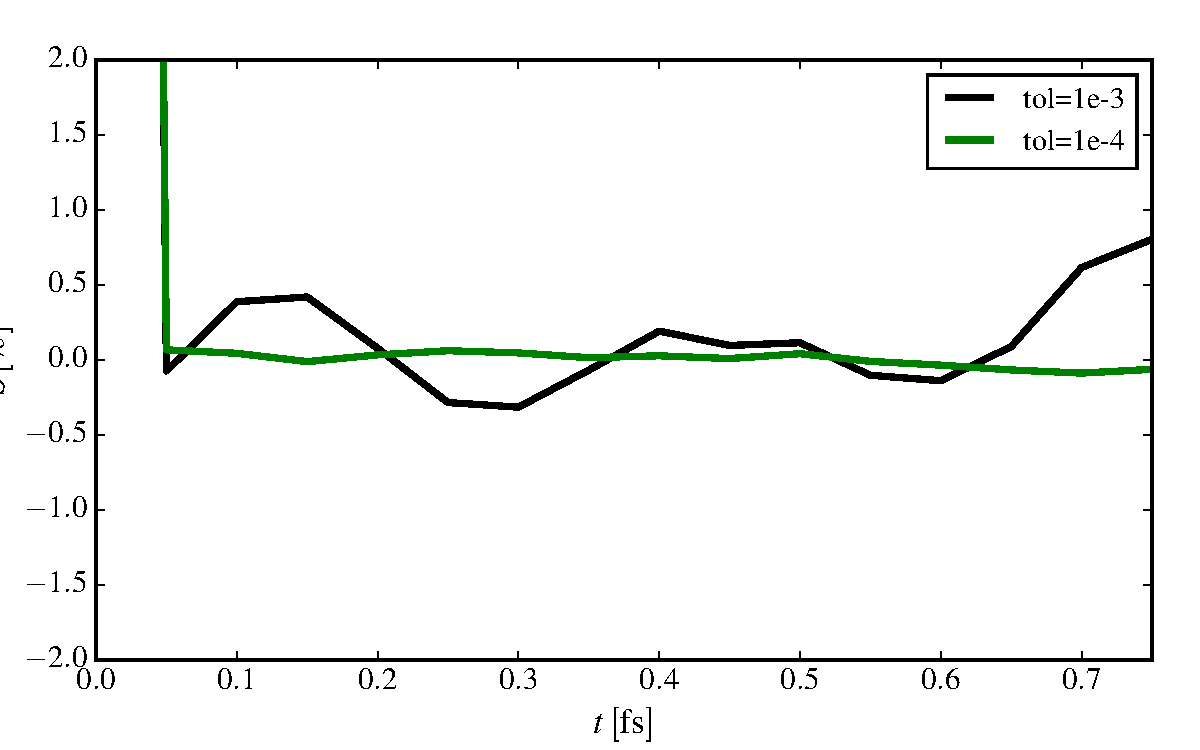
\includegraphics[width=0.8\textwidth]{figs/L1x3_t1_25_tamen_nvib20_SP_V10_tolVar.pdf}
	\caption{$n_\mathrm{vib}=20$.}
\end{figure}
\clearpage
\subsection{Maximal rank}
\begin{figure}[!h]
	\centering
	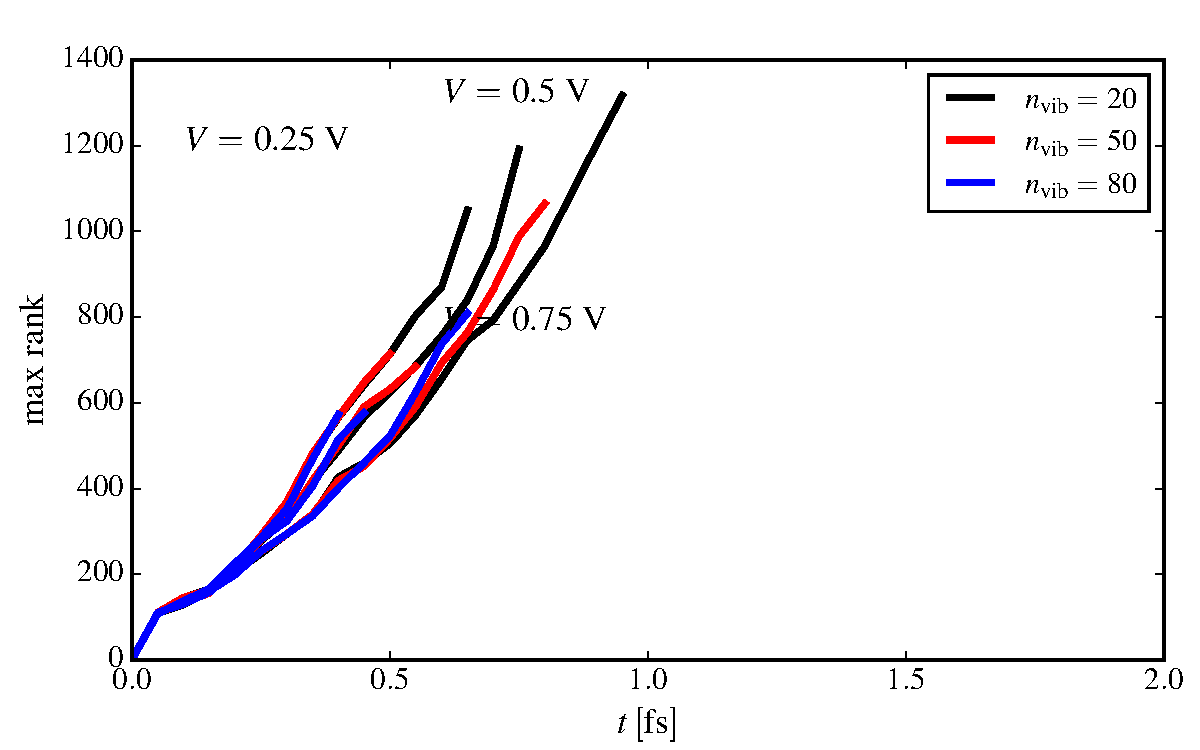
\includegraphics[width=0.75\textwidth]{figs/L1x3_t1_25_tamen_maxRank_P_Vvar_nVar_tol1e-4.pdf}
	\caption{tol$\ =10^{-4}$.}
\end{figure}



\end{document}


